\section{Distributed Instantiation}
\label{sec:system-model}

\begin{figure}[!t]
\centering
\subcaptionbox[] {\small
  Branches $b_1$, $b_2$ and $b_3$ mapped to nodes $n_1$, $n_2$ and
  $n_3$. Each time step captures concurrent operations among the
  nodes.
  \label{fig:instantiation-1}
} [0.47\columnwidth] {
  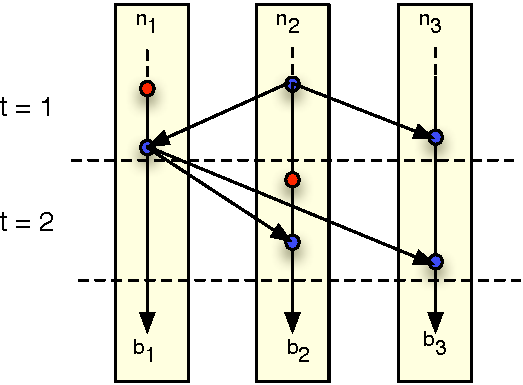
\includegraphics[scale=0.6]{Figures/instantiation-1}
}
\hfill
\subcaptionbox[] {\small
  Network partitions may leave branches $b_1$ and $b_4$ in one
  partition (red background), and branches $b_2$ and $b_3$ in the
  other (yellow background). Since $b_2$ and $b_3$ cannot merge unless
  $b_1$ and $b_4$ merge (Fig.~\ref{fig:legal-extensions}), they cannot
  communicate among themselves even though they are in the same
  network partition.
} [0.47\columnwidth] {
  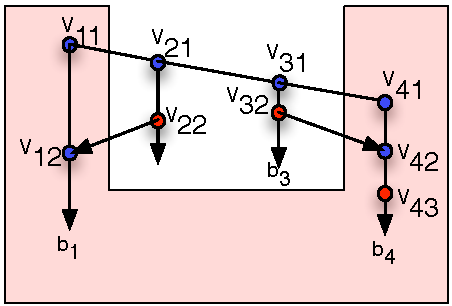
\includegraphics[scale=0.8]{Figures/partitions}
}
\caption{Instantiations of the \name concurrency model in a
distributed setting}
\label{fig:partitions}
\end{figure}

The operational semantics of \name describe a concurrency model based
on versions and branches for computations on replicated data, without
referring to any particular instantiation. A useful instantiation of
the model is for a distributed system with multiple nodes, where each
each node hosts a \emph{replica} of the data. Thus, each node
instantiates a branch. The node responds to user requests to perform
updates to the replica, and publishes the results on its local branch
as newer versions. The node also stores (a prefix of) the branching
history - a knowledge about the system that it accumulates over time.
In response to the publication of a new local version, it contacts
other nodes to obtain their latest local versions, in the process
updating its knowledge about the branching history. If a later version
($v_j$) on a remote branch ($b_j$) is mergeable with the latest
version ($v_i$) on the local branch ($b_i$), i.e., if $v_j \not\preceq
v_i$ and LCA of $b_i$ and $b_j$ is unique, the node initiates the
merge process with the remote node, where in it lets the remote node
know that a new version ($v_i'$) later than $v_i$ is being created on
$b_j$ by merging version $v_j$ of $b_j$. This prevents the remote node
from merging versions $v_i$ or earlier of $b_i$, and creating a
criss-cross branching structure. The later merge of $b_i$ into $b_j$
by the remote node will only consider versions $v_i'$ or later. The
merge operation is a function over participating branches, and occurs
in a single time step, extending one of the branches. Concurrent
merges that do not seek to extend a branch participating in the
current merge operation are allowed. The resultant history of merges
will still be linearizable. The example in
Fig.~\ref{fig:instantiation-1} illustrates. Here, in the time step
$t=1$, nodes $n_1$ and $n_2$ communicate to merge branch $b_2$ in
$b_1$. Concurrently, $n_1$ and $n_3$ can also communicate to merge
$b_2$ into $b_3$. Likewise, at $t=1$, merges from $b_1$ into $b_2$ and
$b_1$ into $b_3$ happen concurrently. The resultant history is
equivalent to performing the merges in the order as they were
described above.

In presence of network partitions, the nodes in one partition may not
receive updates from the other partition, hence merges cannot happen
across a partition. This can be a problem if a pair of branches in one
partition (the current partition) have multiple LCAs in the other
partition (the remote partition), hence cannot merge.
Fig.~\ref{fig:partitions} illustrate this problem for the branching
structure of Fig.~\ref{fig:external-lcas}. Fortunately, the access to
full (causal) branching history at every node comes to the rescue.
Relying on the history, the current partition can fork-off (\C{fork})
new branches that start where the remote branches left, and map them
to new (virtual) nodes that emulate the nodes in the remote partition.
For the example in Fig.~\ref{fig:partitions}, the partition of $b_1$
and $b_4$ can fork new branches $b_2'$ and $b_3'$ from $b_2$ and
$b_3$, respectively, and resume the activity as if the partition never
happened. After merging the first versions on $b_2'$ and $b_3'$,
branches $b_1$ and $b_2$ will be in the same state as before (when the
partition happened), except that the branches are now mergeable
because $b_2'$ and $b_3'$ can merge. The ability to track full
provenance information is thus crucial for \name to overcome network
partitions, making it an appropriate programming model for
highly-available replicated data types.
